Figures~\ref{fig:dr} and~\ref{fig:drmedian} and Table~\ref{tab:dr} show the distance $\Delta R$ (pseudorapidity and
azimuth) between each axis and the truth boson (\code{analysis/axisDeltaR.py}), for jets matched to a truth boson whose
mass lies between 60 and 116\GeV{} (the union of the $W$ and $Z$ windows of Appendix~\ref{app:truth}); without this
requirement, low-mass $\gamma^*\to q\bar q$ ``bosons'' of the \code{ZZto2L2Q} sample, generated down to $4\GeV$, enter.
The sample is 23 files of \code{ZZto2L2Q} (15) and \code{WZto2L2Q} (8), processed with the configuration of this note;
one further \code{ZZto2L2Q} file (707 events) has no selected event. This gives 1743 reco and 1876 gen jets, weighted with
the generator weight.
\begin{itemize}
\item The jet axis is the closest to the boson at every $\pt$: median $\Delta R$ 0.059, 0.027, 0.017 and 0.009 for reco
  jets with $\pt$ 200--300, 300--400, 400--600 and above $600\GeV$. The groomed and trimmed axes are slightly farther
  (by up to 0.006 in the median); not studied further.
\item The winner-take-all axes follow the harder of the two quarks, not the boson: their median distance is 0.18 at
  200--300\GeV{} and falls with $\pt$ like the opening angle of the decay (Eq.~\eqref{eq:app:containment}). The
  Cambridge--Aachen and $k_\mathrm{T}$ versions are indistinguishable.
\item The recoil axis is at a median 0.07--0.10; its azimuth is that of the dilepton system, which also recoils against
  additional radiation (not verified separately).
\item All axes have a tail: 10\% of the jets lie beyond $\Delta R \approx 0.2$ from the boson even for the jet axis.
  At 200--300\GeV, 5\% lie beyond 0.44; jets containing only one of the quarks (Appendix~\ref{app:truth:bias}) are a
  likely source, which has not been checked jet by jet.
\item Soft drop ends on a single particle (status 1) for at most 0.8\% of the jets, and no axis is unavailable
  (status 2) for these truth-matched jets.
\end{itemize}

\begin{figure}[htbp]
\centering
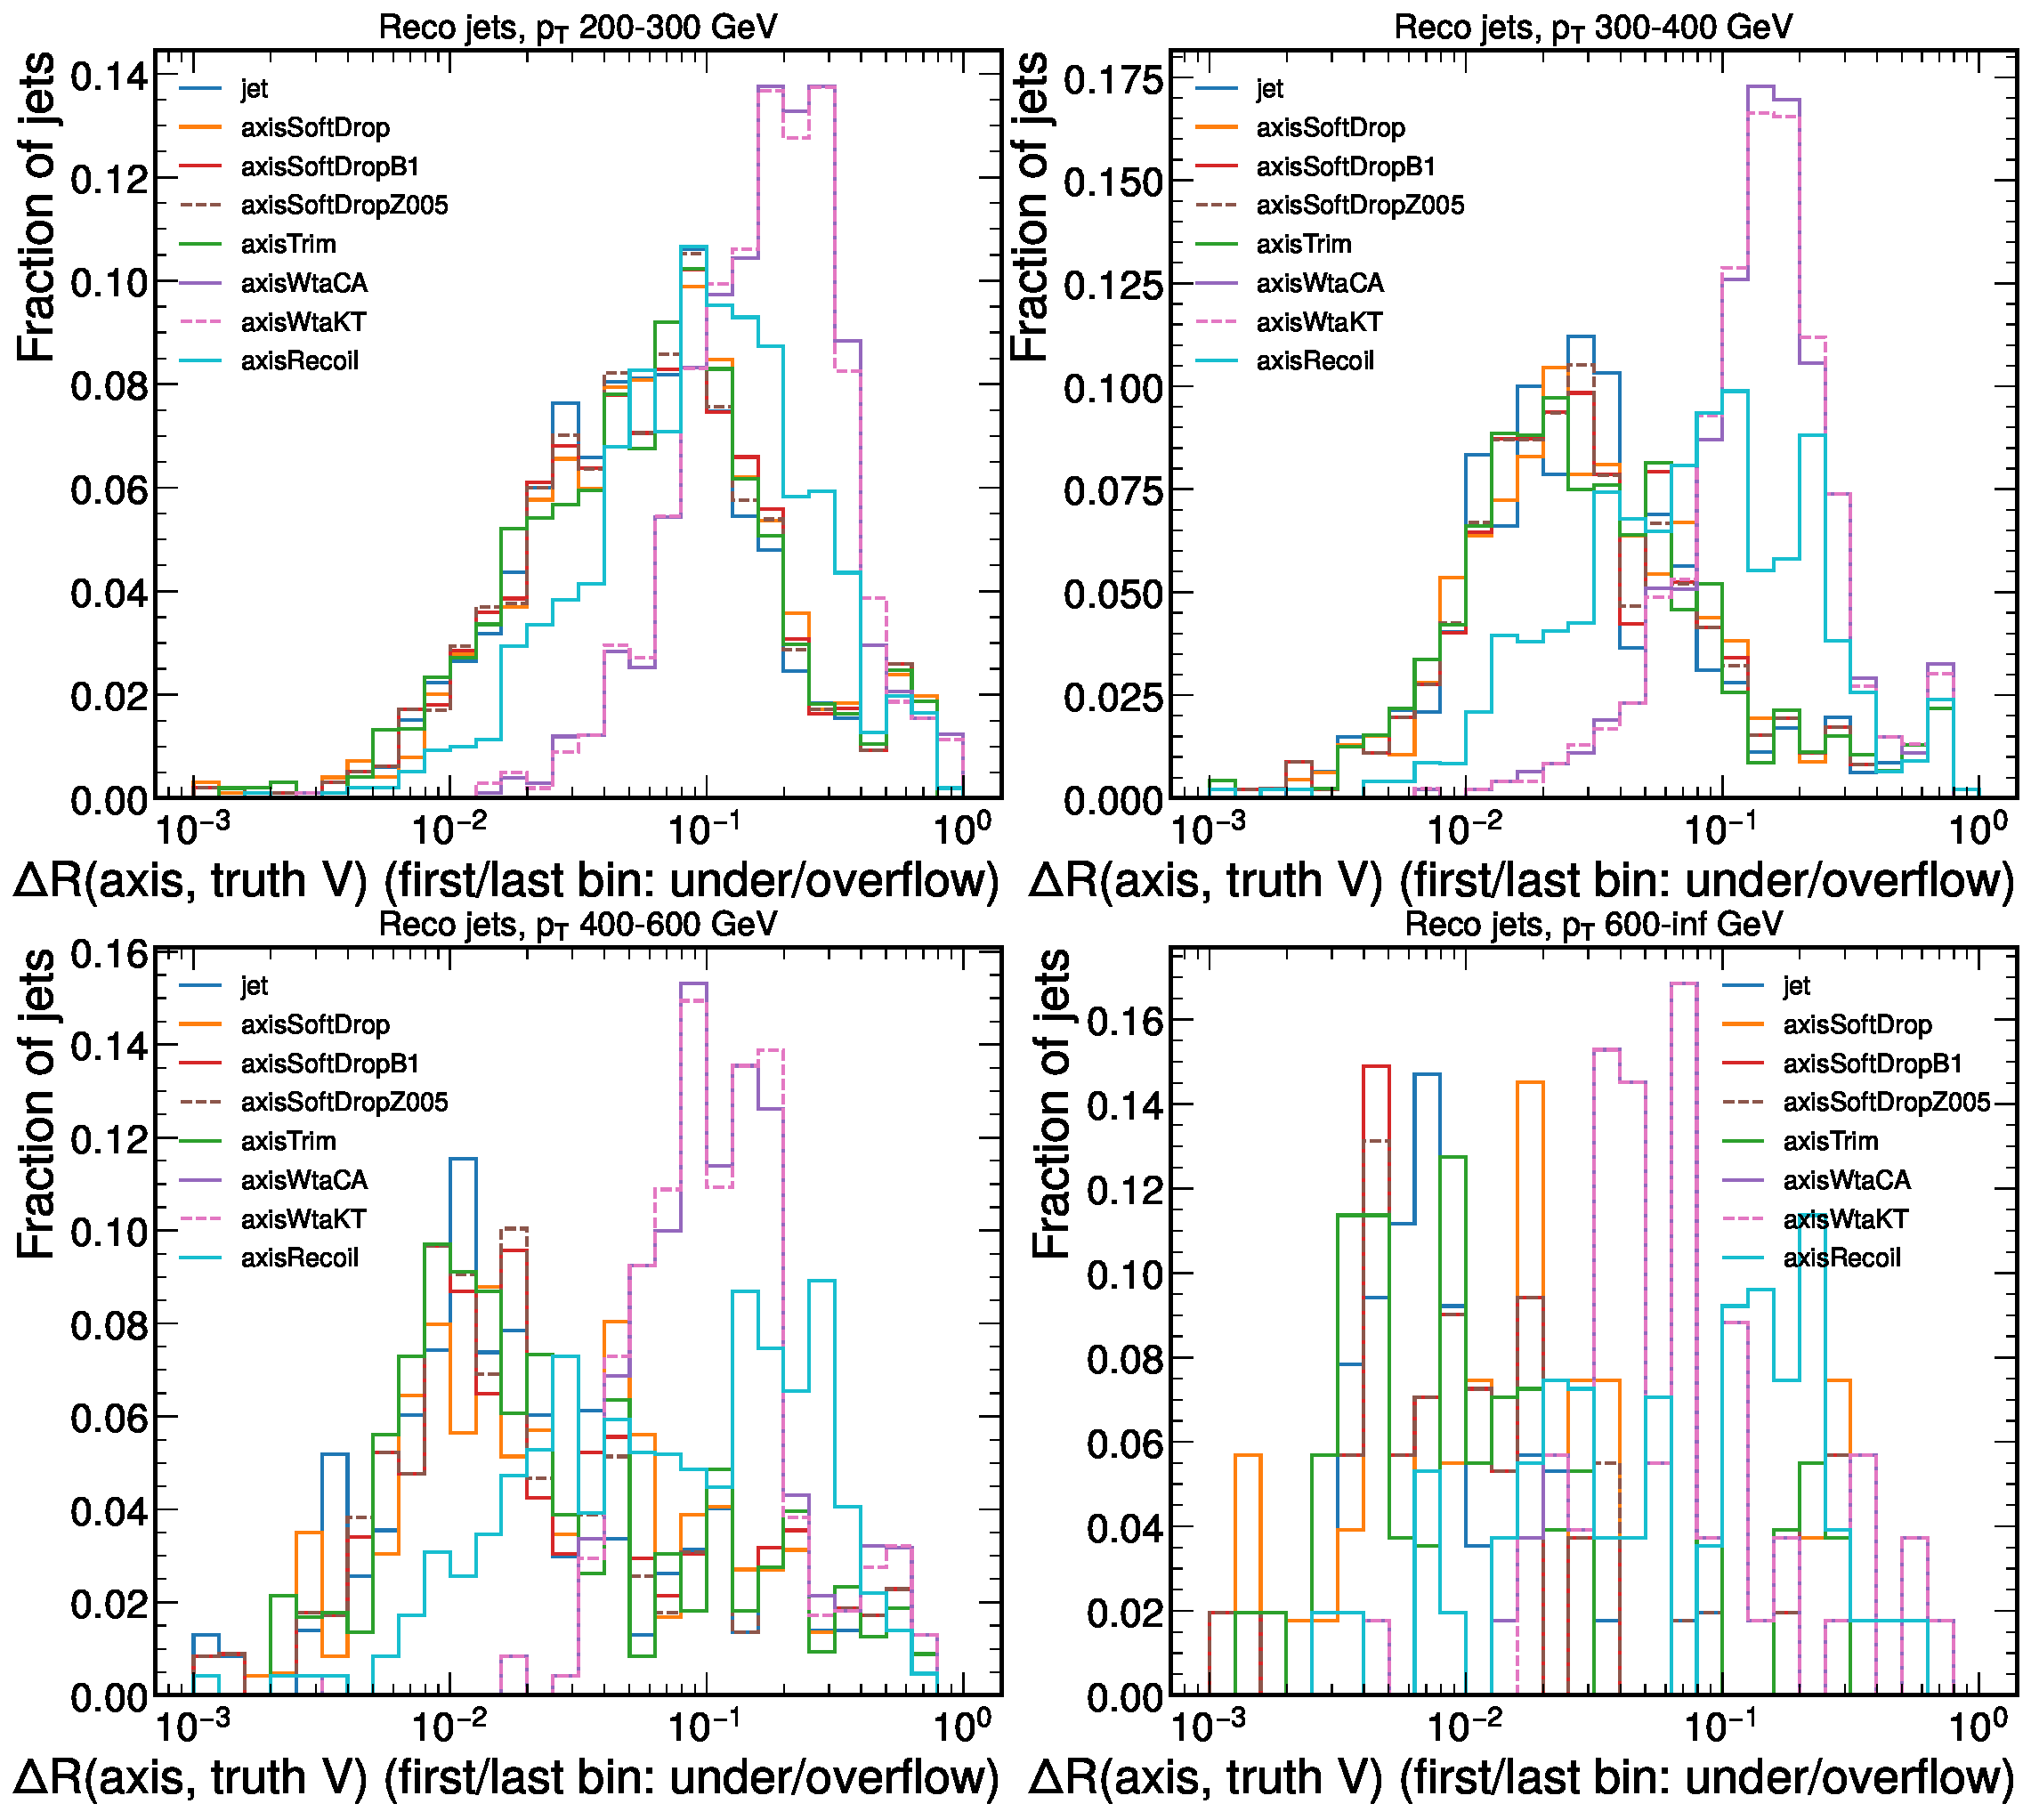
\includegraphics[width=0.49\textwidth]{figures/dR_Reco.pdf}\hfill
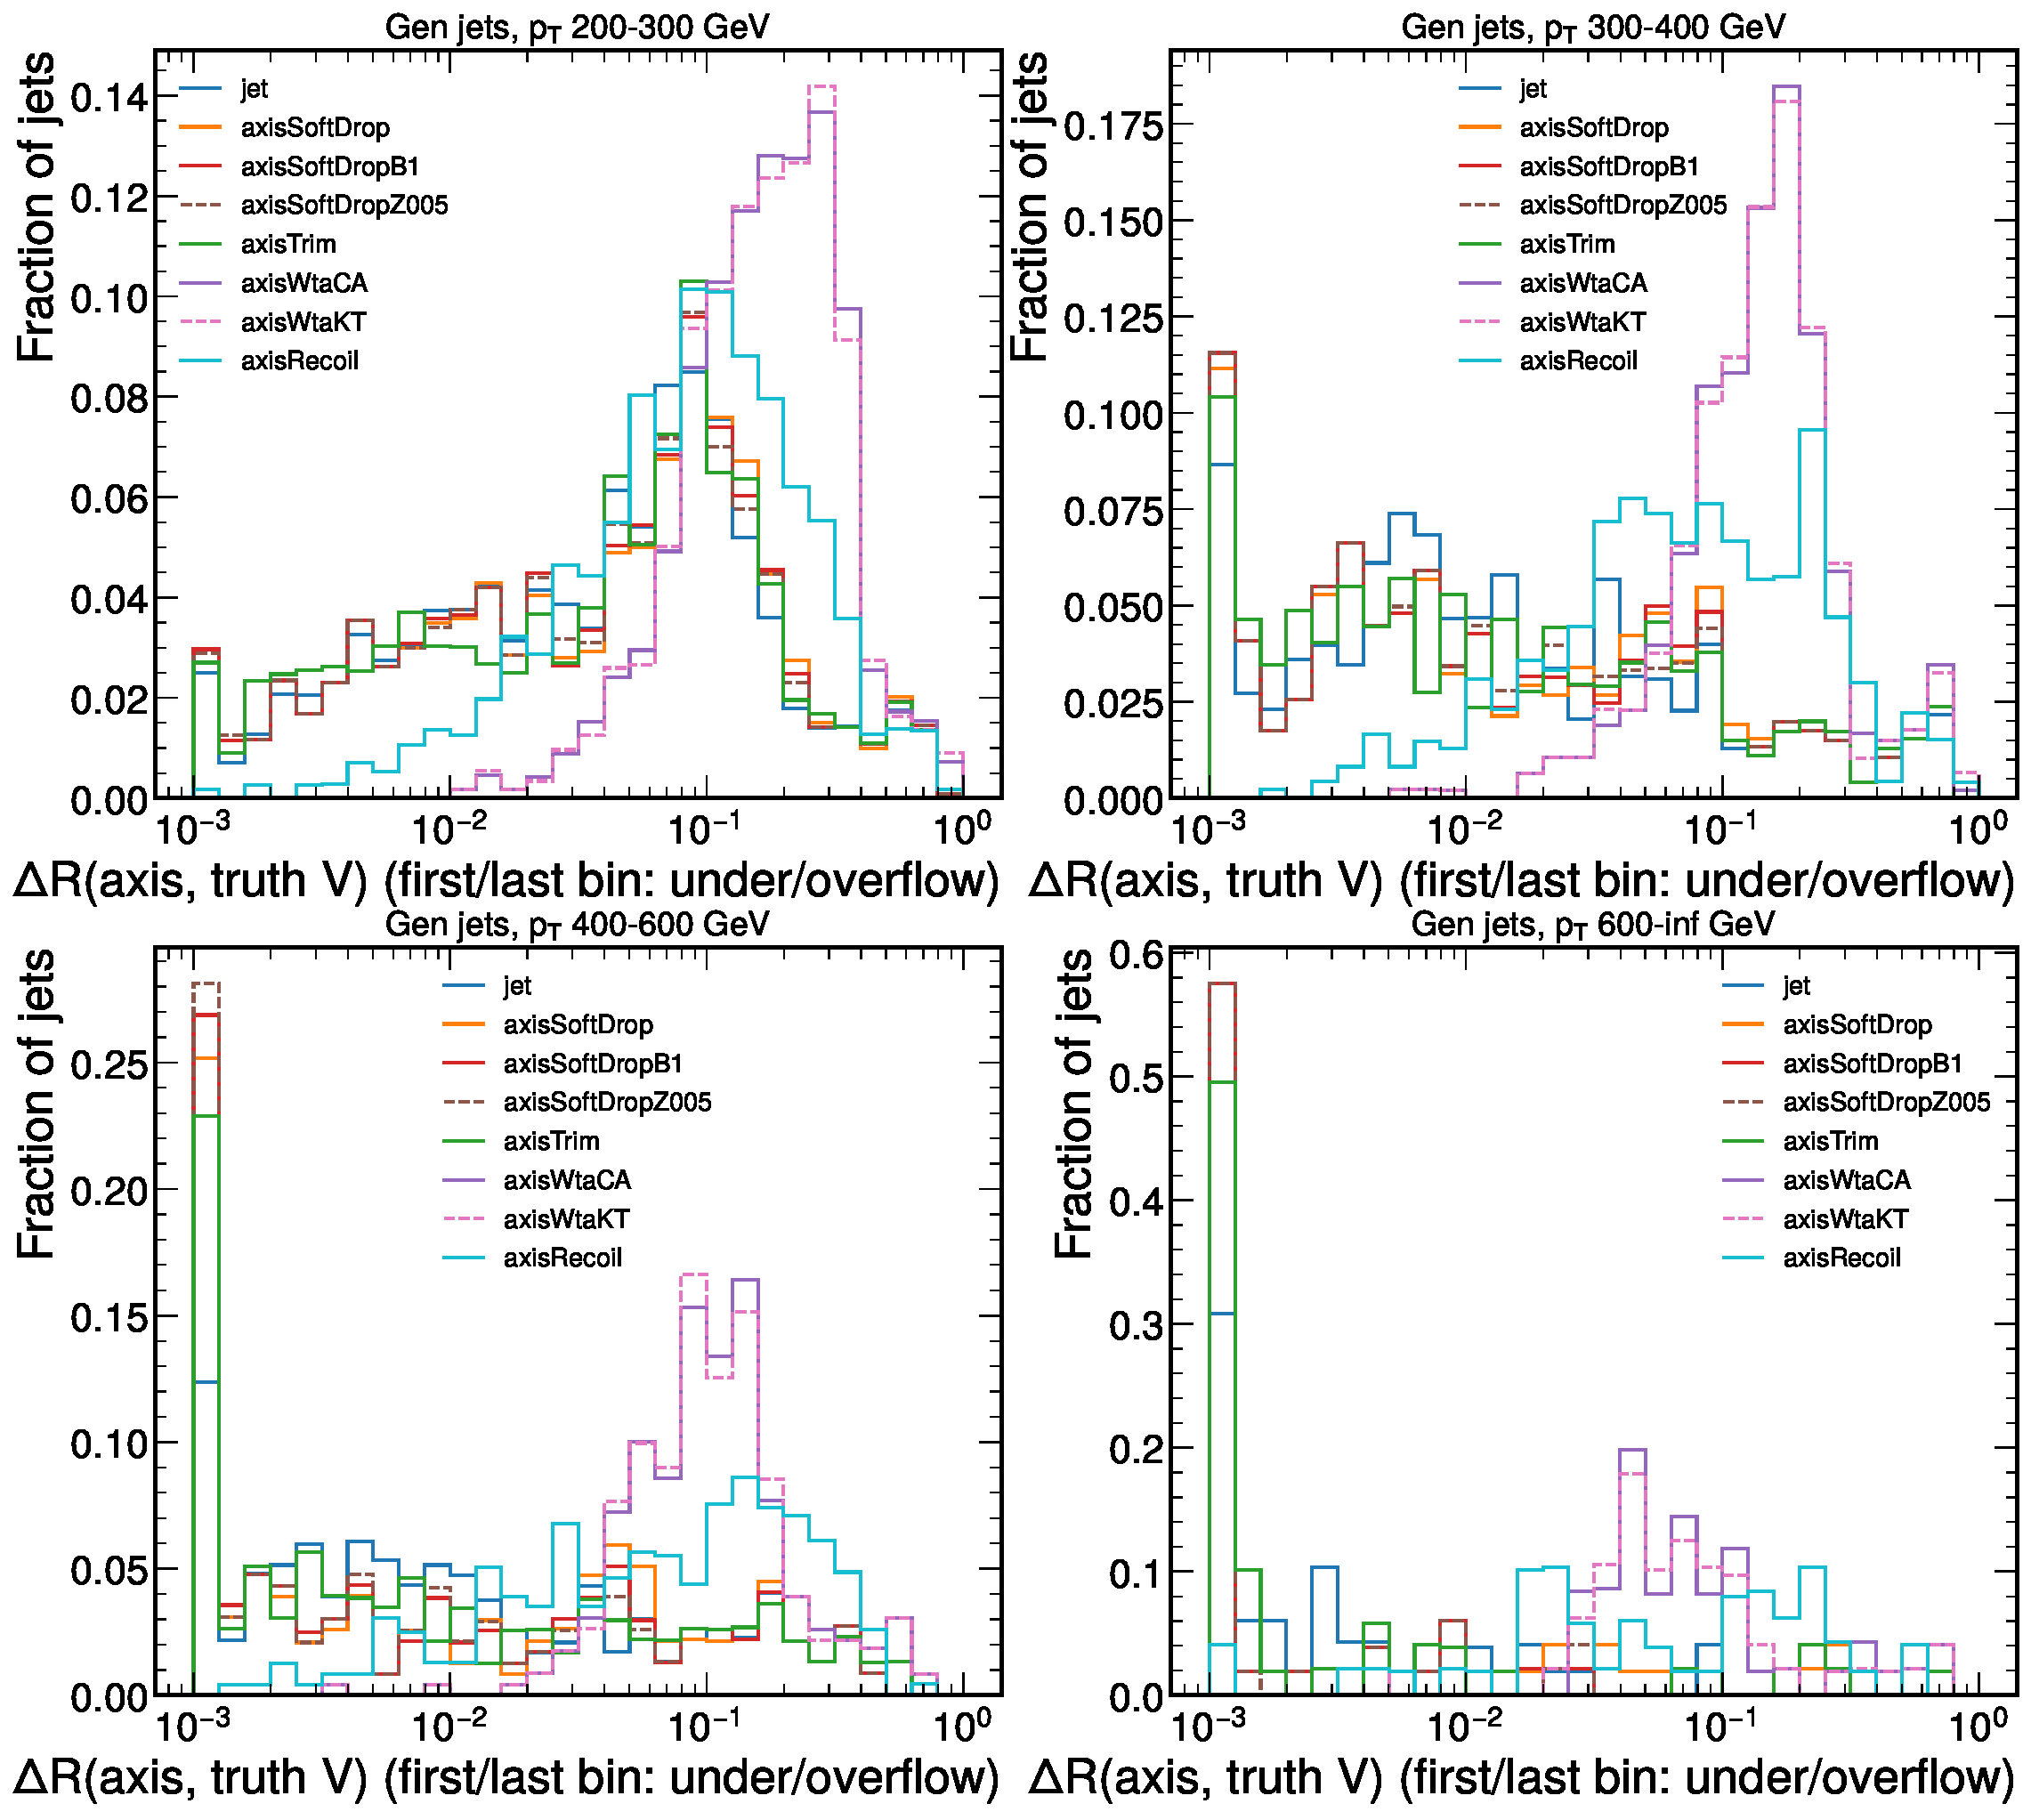
\includegraphics[width=0.49\textwidth]{figures/dR_Gen.pdf}
\caption{Distribution of $\Delta R$ between each axis and the truth boson, normalised to the number of jets, in four bins
of jet $\pt$ (200--300, 300--400, 400--600 and above $600\GeV$), for reco jets (left) and gen jets (right). Logarithmic
bins between $10^{-3}$ and 1; the first and last bins contain the under- and overflow.}
\label{fig:dr}
\end{figure}

\begin{figure}[htbp]
\centering
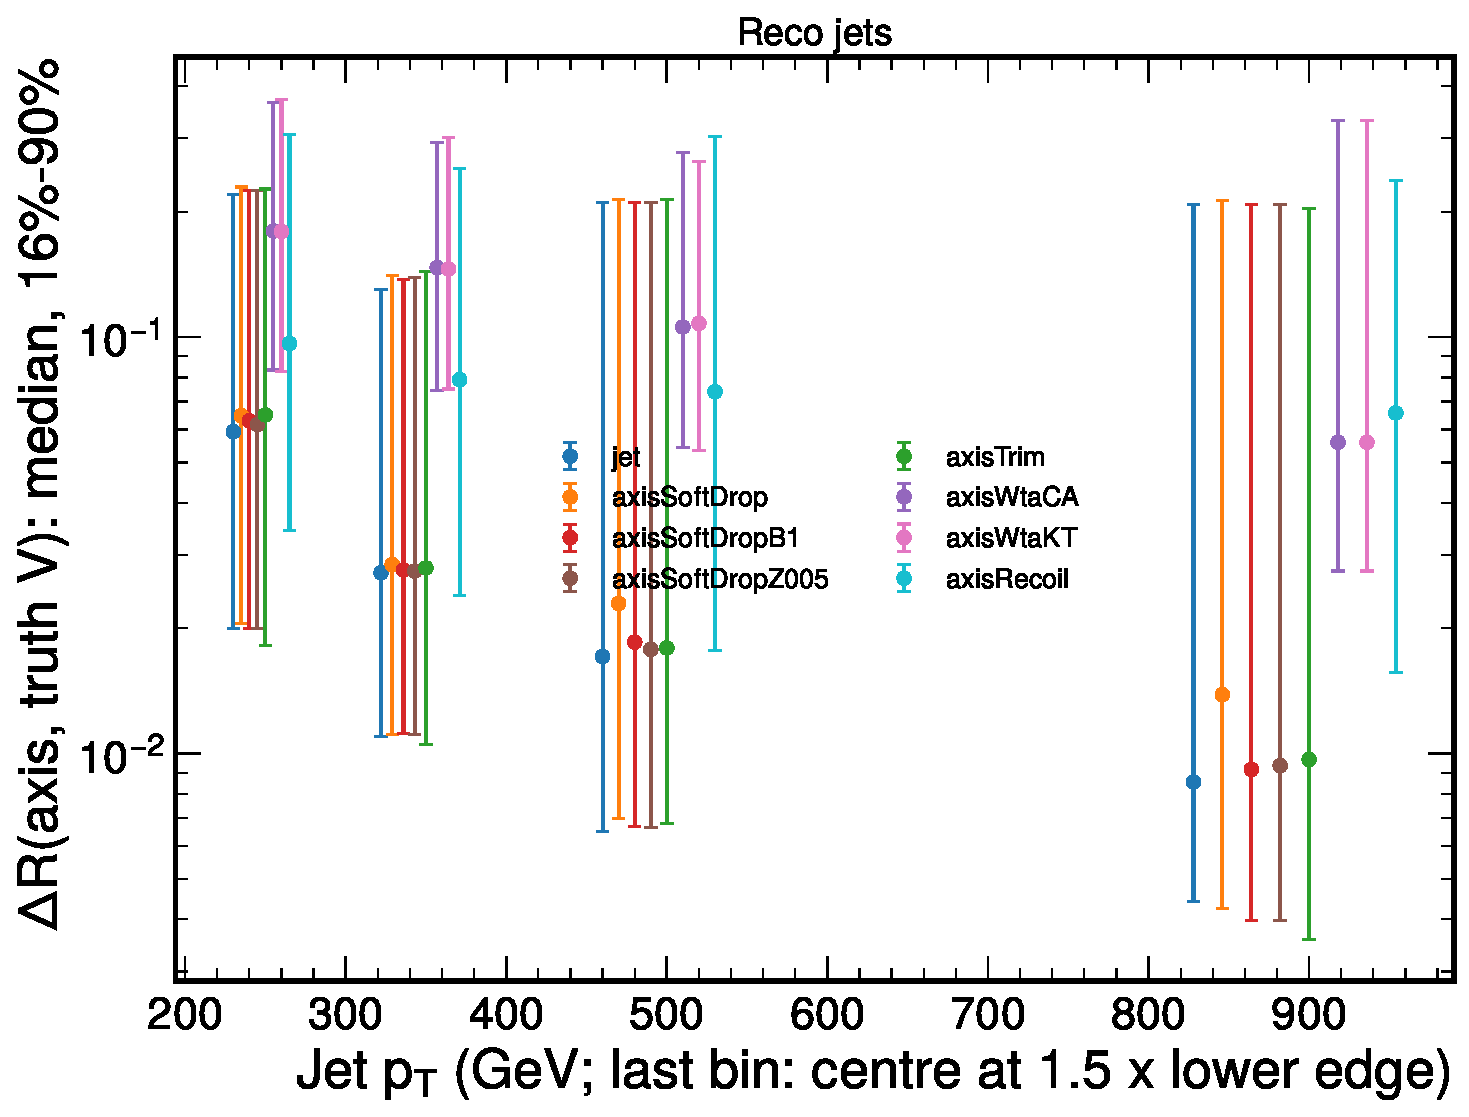
\includegraphics[width=0.49\textwidth]{figures/dRmedian_Reco.pdf}\hfill
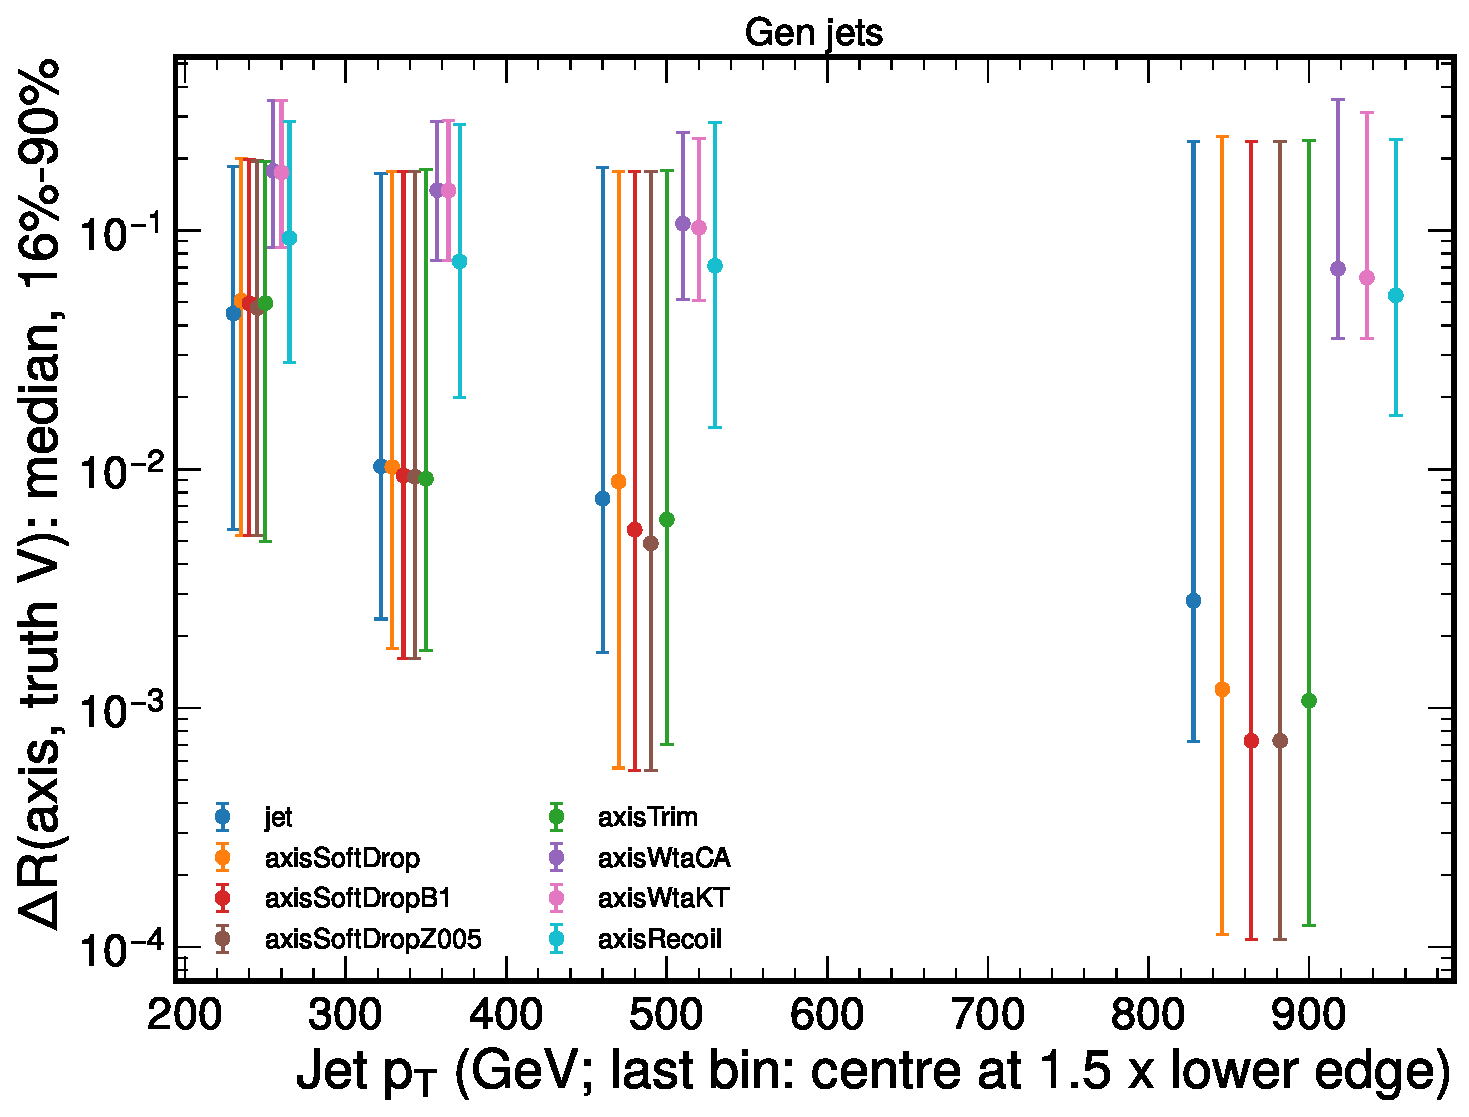
\includegraphics[width=0.49\textwidth]{figures/dRmedian_Gen.pdf}
\caption{Median of $\Delta R$ between each axis and the truth boson versus jet $\pt$ (markers), with the interval
between the 16\% and 90\% quantiles (bars); reco jets (left) and gen jets (right). The markers of each $\pt$ bin are
displaced horizontally for readability.}
\label{fig:drmedian}
\end{figure}

\begin{table}[htbp]
\centering
\caption{Median and 90\% quantile of $\Delta R$(axis, truth boson), and the fraction of jets with $\Delta R < 0.05$, per
bin of jet $\pt$. Reco jets: 990, 470, 229 and 54 jets per bin; gen jets: 1124, 472, 231 and 49. The full tables, with
the mean and the 68\% and 95\% quantiles, are in \code{dR.md} of the study directory.}
\label{tab:dr}
\footnotesize
\setlength{\tabcolsep}{3pt}
\begin{tabular}{lcccccccccccc}
\toprule
 & \multicolumn{3}{c}{200--300\GeV} & \multicolumn{3}{c}{300--400\GeV} & \multicolumn{3}{c}{400--600\GeV} & \multicolumn{3}{c}{$> 600\GeV$} \\
axis & q50 & q90 & $f_{<0.05}$ & q50 & q90 & $f_{<0.05}$ & q50 & q90 & $f_{<0.05}$ & q50 & q90 & $f_{<0.05}$ \\
\midrule
\multicolumn{13}{l}{\emph{reco jets}} \\
jet & 0.059 & 0.22 & 0.44 & 0.027 & 0.13 & 0.71 & 0.017 & 0.21 & 0.74 & 0.009 & 0.21 & 0.81 \\
soft drop & 0.065 & 0.23 & 0.41 & 0.028 & 0.14 & 0.68 & 0.023 & 0.21 & 0.68 & 0.014 & 0.21 & 0.81 \\
soft drop $\beta=1$ & 0.063 & 0.22 & 0.43 & 0.028 & 0.14 & 0.68 & 0.018 & 0.21 & 0.72 & 0.009 & 0.21 & 0.81 \\
soft drop $z_\mathrm{cut}=0.05$ & 0.062 & 0.23 & 0.43 & 0.027 & 0.14 & 0.69 & 0.018 & 0.21 & 0.73 & 0.009 & 0.21 & 0.81 \\
trimming & 0.065 & 0.23 & 0.42 & 0.028 & 0.14 & 0.69 & 0.018 & 0.21 & 0.74 & 0.010 & 0.20 & 0.81 \\
WTA C/A & 0.180 & 0.37 & 0.06 & 0.147 & 0.29 & 0.08 & 0.106 & 0.28 & 0.12 & 0.056 & 0.33 & 0.45 \\
WTA $k_\mathrm{T}$ & 0.179 & 0.37 & 0.06 & 0.146 & 0.30 & 0.07 & 0.108 & 0.26 & 0.12 & 0.056 & 0.33 & 0.45 \\
recoil & 0.097 & 0.31 & 0.25 & 0.079 & 0.25 & 0.35 & 0.074 & 0.30 & 0.41 & 0.066 & 0.24 & 0.42 \\
\midrule
\multicolumn{13}{l}{\emph{gen jets}} \\
jet & 0.045 & 0.18 & 0.52 & 0.010 & 0.17 & 0.77 & 0.007 & 0.18 & 0.76 & 0.003 & 0.24 & 0.81 \\
soft drop & 0.051 & 0.20 & 0.50 & 0.010 & 0.18 & 0.72 & 0.009 & 0.18 & 0.73 & 0.001 & 0.25 & 0.80 \\
soft drop $\beta=1$ & 0.050 & 0.20 & 0.50 & 0.009 & 0.18 & 0.72 & 0.006 & 0.18 & 0.76 & 0.001 & 0.24 & 0.81 \\
soft drop $z_\mathrm{cut}=0.05$ & 0.047 & 0.20 & 0.51 & 0.009 & 0.18 & 0.75 & 0.005 & 0.18 & 0.76 & 0.001 & 0.24 & 0.81 \\
trimming & 0.050 & 0.19 & 0.51 & 0.009 & 0.18 & 0.75 & 0.006 & 0.18 & 0.76 & 0.001 & 0.24 & 0.81 \\
WTA C/A & 0.178 & 0.35 & 0.06 & 0.147 & 0.29 & 0.08 & 0.107 & 0.26 & 0.14 & 0.069 & 0.35 & 0.37 \\
WTA $k_\mathrm{T}$ & 0.175 & 0.35 & 0.06 & 0.147 & 0.29 & 0.08 & 0.102 & 0.24 & 0.14 & 0.063 & 0.31 & 0.37 \\
recoil & 0.093 & 0.28 & 0.28 & 0.074 & 0.28 & 0.38 & 0.071 & 0.28 & 0.40 & 0.053 & 0.24 & 0.49 \\
\bottomrule
\end{tabular}
\end{table}
